\section{Evaluation}

We built \tool ($\sim$20K lines of code in Java) upon Sysdig~\cite{sysdig}, 
and evaluate \tool using both the attack cases constructed based on the known exploits~\cite{exploitdb,liu2018priotracker,kwon2018mci,reduction} and the attack cases collected by the DARPA Transparent Computing (TC) program~\cite{tc}.
In the evaluations, we aim to answer the following research questions:

\begin{itemize}[noitemsep, topsep=1pt, partopsep=1pt, listparindent=\parindent, leftmargin=*]
% \begin{itemize}
\item \textbf{RQ1}: How effective is \tool in revealing attack sequences in comparison with other state-of-art techniques? 
\item \textbf{RQ2}: How many top-ranked entry nodes should be used in \tool for revealing attack sequences?
\item \textbf{RQ3}: How effective is \tool in revealing attack entries?
\item \textbf{RQ4}: How efficient is \tool in investigating an attack?
\end{itemize}

% RQ1 aims to measure the effectiveness of using only weights for graph reduction.
% Its results will provide motivation for the design of \tool.
%  Its result evaluate the effectiveness of \tool for dependency graph reduction, which plays an essential role in addressing the challenges mentioned in \cref{sec:intro}.

% RQ1 aims to evaluate the overall effectiveness of \tool in dependency graph reduction, and compare \tool with other state-of-the-art causality analysis techniques.
% RQ2 aims to evaluate how the top-ranked entry nodes affect the effectiveness of \tool.
% RQ3 aims to evaluate whether \tool consistently ranks the attack entries 
% upfront, and compare \tool with other baseline approaches.
% RQ4 aims to measure the execution times of \tool and its variation, and compare \tool with other state-of-the-art causality analysis techniques.

\begin{table*}[!htb]
\centering
\ra{1.2}
\caption{Statistics of dependency graphs generated for all the 15 attacks}
\label{tab:stasticalSummary}
\resizebox{\textwidth}{!}{
\begin{tabular}{@{}crrrrrrrr@{}}
\toprule
\textbf{Attack}      & \multicolumn{1}{c}{\textbf{Causality Analysis \# V}} & \multicolumn{1}{c}{\textbf{Causality Analysis \# E}} & \multicolumn{1}{c}{\textbf{Edge Merge \#V}} & \multicolumn{1}{c}{\textbf{Edge Merge \# E}} & \multicolumn{1}{c}{\textbf{Entry Nodes}} & \multicolumn{1}{c}{\textbf{Critical Edge}} & \multicolumn{1}{c}{\textbf{Attack Entries}} & \multicolumn{1}{c}{\textbf{POI}} \\ \midrule
Wget Executable      & 126                                               & 673                                               & 126                                      & 363                                       & 46                                    & 8                                       & 2                                        & $\sim$50MB                       \\
Illegal Storage      & 8,450                                             & 93,085                                            & 8,450                                    & 62,073                                    & 960                                   & 6                                       & 2                                        & $\sim$50MB                       \\
Illegal Storage2     & 42,450                                            & 658,913                                           & 42,450                                   & 378,326                                   & 3,499                                 & 4                                       & 2                                        & $\sim$50MB                       \\
Hide File            & 194,208                                           & 6,464,098                                         & 194,208                                  & 3,273,769                                 & 35,203                                & 12                                      & 2                                        & $\sim$50MB                       \\
Steal Information    & 195,636                                           & 6,493,626                                         & 195,636                                  & 3,291,208                                 & 35,213                                & 4                                       & 2                                        & $\sim$50MB                       \\
Backdoor Download    & 7,510                                             & 69,479                                            & 7,510                                    & 60,390                                    & 157                                   & 8                                       & 2                                        & $\sim$50MB                       \\
Annoying Server User & 114                                               & 585                                               & 114                                      & 318                                       & 34                                    & 10                                      & 2                                        & $\sim$50MB                       \\
Shellshcok           & 1,648                                             & 20,332                                            & 1,648                                    & 3,600                                     & 1,273                                 & 30                                      & 3                                        & 124B                             \\
Dataleak             & 407                                               & 2,262                                             & 407                                      & 1,152                                     & 234                                   & 18                                      & 3                                        & 7.1KB                            \\
VPN Filter           & 1,195                                             & 5,212                                             & 1,195                                    & 1,879                                     & 999                                   & 10                                      & 2                                        & 1.6KB                            \\
Five Dir Case1       & 240                                               & 272                                               & 240                                      & 272                                       & 232                                   & 2                                       & 1                                        & 50.78KB                          \\
Five Dir Case3       & 5,907                                             & 78,075                                            & 5,907                                    & 78,075                                    & 879                                   & 4                                       & 1                                        & 121.85KB                         \\
Theia Case1          & 184,352                                           & 816,277                                           & 184,352                                  & 816,277                                   & 151,827                               & 8                                       & 2                                        & 166.78KB                         \\
Theia Case3          & 334,441                                           & 1,500,717                                         & 334,441                                  & 1,500,717                                 & 282,651                               & 6                                       & 2                                        & 166.64KB                         \\
Trace Case5          & 263                                               & 971                                               & 263                                      & 971                                       & 28                                    & 3                                       & 1                                        & 95.KB                            \\
\textbf{AVG}         & 65,129.80                                            & 1,080,305.13                                         & 65,129.80                                   & 631,292.67                                   & 34,215.67                                & 8.87                                       & 1.93                                        & --                               \\ \bottomrule
\end{tabular}
}
\end{table*}

\subsection{Evaluation Setup}
\label{subsec:evalsetup}
We deployed Sysdig~\cite{sysdig} on 5 Linux hosts to collect system auditing events and then applied \tool to perform attack investigation. 
\tool is executed on a server with an Intel(R) Xeon(R) CPU E5-2637 v4 (3.50GHz), 256GB RAM running 64bit Ubuntu 18.04.1.
For investigating the attack cases based on the known exploits, we performed 10 attacks in the deployed environment: 7 attacks based on commonly used exploits and 3 multi-host and mutli-step intrusive attacks based on the Cyber Kill Chain framework~\cite{cyberkillchain} and CVE reports~\cite{cve}.
The deployed hosts have 12 active users with hundreds of processes, and are used for various types of daily tasks such as file manipulation, text editing, and software development, which are representative of real-world usage.
During evaluation, the deployed hosts continue to resume their routine tasks to emulate the real-world deployment where irrelevant system activities and attack activities co-exist.
The routine tasks on these machines ensure that enough noise of irrelevant system activities is collected.
In total, the real system audit logs collected in our deployed hosts contain \emph{$\sim$100 million} events. 
The DARPA dataset includes system audit logs collected from 5 hosts with different OS systems.
We developed a tool to parse the released logs and loaded the events into our databases.
In total, the DARPA dataset used in our evaluation contains \emph{$\sim$50 million} events.
We next describe these attacks in detail. 




% We performed a series of attacks based on known exploits~\cite{exploitdb,liu2018priotracker,kwon2018mci,reduction} in the deployed environment, and applied \tool to 
% investigate these attacks, demonstrating the effectiveness of \tool.
% We then collected system auditing events for the attacks and applied \tool to analyze events. 
% There are five more attacks performed by researchers of DARPA transparent computing program (DARPA TC).






\subsubsection{Attacks Based on Commonly Used Exploits}
\label{subsub:benign-cases}
These 7 attacks are used in prior work's evaluations~\cite{exploitdb,liu2018priotracker,kwon2018mci,reduction},
which consist of the following scenarios: 
\begin{itemize}[noitemsep, topsep=1pt, partopsep=1pt, listparindent=\parindent, leftmargin=*]
    \item \textit{Wget Executable}: A vulnerable server allows the attacker to download executable files using wget. 
    The attacker downloads python scripts and executes the scripts.
    \item \textit{Illegal Storage}: A server administrator uses wget to download suspicious files to a user's home directory.
    \item \textit{Illegal Storage 2}: A server administrator uses curl to download suspicious files to a user's home directory.
    \item \textit{Hide File}: The goal of the attacker is to hide malicious file among the user's normal files. 
    The attacker downloads the malicious script and hides it by changing its file name and location.
    \item \textit{Steal Information}: The attacker steals the user's sensitive information and writes the information to a hidden file.
    \item \textit{Backdoor Download}: A malicious insider uses the ping command to connect to the malicious server, and then downloads the backdoor script from the server and hides the script by renaming it.
    \item \textit{Annoying Server User}: 
    %A vulnerable server is used by multiple users. 
    The annoying user logs into other user's home directories on a vulnerable server and writes some garbage data to other user's files. 
\end{itemize}


\subsubsection{APT Attacks}
\label{subsubsec:attack-cases}

We performed five APT attacks that capture the important traits of APT attacks depicted from the Cyber Kill Chain framework~\cite{cyberkillchain}. 
Note that an APT attack consists of a series of steps, and some steps may not be captured by system monitoring (\eg user inputs and inter-process communications).
Such limitations can be addressed by employing more powerful auditing tools, but it is out of the scope of this paper.
Thus, we identified 10 key steps that are related to POI entities for our evaluations in the five APT attacks.


\myparatight{APT Attack 1: Zero-Day Penetration to Target Host}
The scenario emulates the attacker's behavior who penetrates the victim's host
leveraging previously unknown Zero-day attack. Zero-day vulnerabilities are
attack vectors that previously unknown to the community, therefore allow the
attacker to put their first step into their targets. In our case, we assume that
the {\tt bash} binary in victim's host is outdated and vulnerable to shellshock~\cite{shellshock}. The victim computer hosts web service that has
CGI written as BASH script. The attacker can run an arbitrary command when she
passes the specially crafted attack string as one of environment variable. Leveraging the vulnerability, the attacker runs a series of remote commands to
plant and run initial attack by: (1) transferring the payload (\emph{penetration-c1}), (2) changing its permission, and (3) running the payload to bootstrap its campaign (\emph{penetration-c2}).
% As a lateral movement, the
% attacker downloads (4) a password cracker program from outside run it against
% the shadow password files. 


\myparatight{APT Attack 2: Password Cracking After Shellshock Penetration}
% Once breaks into the system, the attacker can launch different malicious
% behaviors (\eg password cracking, information leakage, denial of services). 
After initial shellshock penetration, the attacker first connects to Cloud services (\eg
Dropbox, Twitter) and downloads an image where C2 (Command and Control) host's IP address is encoded in EXIF metadata (\emph{password-crack-c1}). The behavior is a common practice shared by APT attacks~\cite{hammertoss,vpnfilter} to evade the network-based detection system based on DNS blacklisting.

Using the IP, The malware connects to C2 host. C2 host directs the malware to take
some lateral movements, including a series of stealthy reconnaissance maneuvers. 
In this stage, the attacker generally takes a number of actions. Among those, we emulate the password cracking attack. The attacker downloads password cracker payload (\emph{password-crack-c2}) and runs it against password shadow files (\emph{password-crack-c3}).

\myparatight{APT Attack 3: Data Leakage After Shellshock Penetration}
After lateral movement stage, the attacker attempts to steal all the valuable assets from the host. 
This stage mainly involves the behaviors of local and remote file system scanning activity, copying and compressing of important files, and transferring to its C2 host.
The attacker scans the file system, scrap files into a single compress file and transfer it back to C2 host (\emph{data-leakage}).

\myparatight{APT Attack 4: Command-line Injection with Input Sanitization Failures}
Different from the previous shellshock case, a program may contain vulnerabilities introduced by developer errors and this can also be a initial attack vector that invites the attacker into their target systems. To represent
such cases, we wrote an web application prototype that fails to sanitize inputs for a certain web request, hence allows Command line Injection attack. 
Our prototype service mimics the Jeep-Cherokee attack case~\cite{miller:remote:2015} which implements a remote access using the conventional web service API that
internally uses DBUS service to run the designated commands. 
Due to the developer mistake, the web service fails to sanitize the remote inputs, the attacker can append arbitrary commands followed by semi-colon({\tt;}). 
Leveraging this vulnerability, we can download backdoor program (\emph{commend-injection-c1}) and collect sensitive data (\emph{command-injection-c2}).

\myparatight{APT Attack 5: VPNFilter}
We prototyped a famous IoT attack campaign; VPNFilter malware~\cite{vpnfilterschenier}, which infected millions of dozens of different IoT devices exploiting a number of
known or zero-day vulnerabilities~\cite{vpnfilter1,vpnfilter2}. The attack's
significance lies in how the malware operates during its lateral movement stage following its initial penetration. 
The campaign employs up-to-date hacker practices to bypass conventional security solutions based on static blacklisting approaches and has an architecture to download plug-in payload on-demand, at run-time. 
We prototyped the malware referring to one of its sample for x86 architecture~\cite{vpnfilterx86}. 

The VPNFilter stage 1 malware accesses a public image repository to get an image. In the EXIF metadata of the image, it contains the IP address for the stage 2 host (\emph{vpnfilter-c1}). It downloads the VPNFilter stage2 from the stage2 server, and runs it (\emph{vpnfilter-c2}).



\subsubsection{DARPA TC Attack Cases}
The dataset released by the DARPA TC program contains attack cases performed on different operating systems.
Based on the attack descriptions provided in the dataset, we exclude the attack cases that fail to launch the attacks, and the attack cases on the Android system since mobile applications' behaviors are constrained by the Android sandbox and are not suitable for our analysis.
We also exclude the phishing e-mail attacks since most of their operations are through clicking links in the browsers and leave limited traces in the system audit logs.
In total, we chosen five attacks that target at different operating systems (Linux, Windows) and exploit different vulnerabilities (Firefox backdoor and browser extensions). 

% Once we got the dependency graph of the malicious behavior, we used \tool to further process and detect the critical component of each attack.



\subsubsection{Obtaining Ground Truth for the Attacks}
For the attack cases performed on our hosts, we identified the POI events based on the performed attacks and applied backward causality analysis from the POI events to obtain the system dependency graphs.
For the attack cases in the DARPA dataset, we queried the databases that are loaded with the logs to identify the POI events based on the attack description, and applied backward causality analysis from the POI events to obtain the system dependency graphs.
For the attacks involving multiple hosts, \tool performs cross-host causality analysis based on the existing techniques~\cite{liu2018priotracker,backtracking2},
which produces causality graphs that include special network connection edges to represent connections among multiple hosts.
% These connection edges ensure that the dependency flows are not cut off across hosts. 
Finally, within our best efforts, we manually ensured that the critical edges and the attack entries were identified based on the knowledge of the performed attacks and the attack descriptions in these system dependency graphs.


\cref{tab:stasticalSummary} shows the statistics of the generated dependency graphs for the attacks. 
Columns ``Causality Ana. \# V'' and ``Causality Ana. \# E'' show the number of nodes and edges after performing the causality analysis from the POI events.
Columns ``Edge Mer. \# V'' and ``Edge Mer. \# E'' show the number of nodes and edges after applying edge merges (\cref{subsubsec:edge-merge}).
Columns ``Entry Nodes'' and  ``Critical Edge'' show the number of entry nodes and critical edges of the dependency graphs. 
Column ``Attack Entries'' shows the number of entry nodes that are labelled as attack entries.
Column ``POI'' shows the data size of the files in the POI events.
%
We clearly observe that even after edge merges, there still remains a large number of edges in the dependency graphs ($631$K on average with the max being $3.3$ million edges), which motivates the further pruning provided by \tool.
Moreover, in these $15$ attacks, the files in the POI events have diversified sizes, ranging from $124$ bytes to $~50M$ bytes, and on average, there are $42,757$ edges (with the max being $962,706$) that have similar data sizes as the files in the POI events.
Thus, directly using the data flow amount to reveal attack sequences will include lots of irrelevant edges in the results, which motivates \tool to combine multiple features for computing edge weights to achieve better performance.


\myparatight{Evaluation Metrics}
\eat{
To measure the missing of critical edges, we compute the \emph{missing rate} $M_{miss} = N_{miss} / N_{critical}$, where $N_{miss}$ represents the number of missing critical edges and $N_{critical}$ represents the total number of critical edges (Column ``Critical Edge'' in \cref{tab:stasticalSummary}).
To measure the impacts of the top-ranked entry nodes, we show the edge number of the critical component \tool in \cref{fig:rq2edge}.}
Besides measuring false positives (detected edges that are not critical edges) and false negatives (missing edges that are critical edges), we compute the false negative rate $FNR = FN / E_{c}$, where $FN$ represents the number of false positives and $E_{c}$ represents the number of critical edges (Column ``Critical Edge'' in \cref{tab:stasticalSummary}),
and the false positive rate $FPR = FP/E_{total}$, where $FP$ represents the number of false positives and $E_{total}$ represents the number of edges from the Column ``Edge Merge \# E'' in \cref{tab:stasticalSummary}.



% These  cover a wide range of POI's size, from several kilobytes to $~50$ megabytes.



% \begin{table}[t]
% \centering
% \ra{1.2}
% \caption{Statistics of dependency graphs generated for the 15 attacks}
% \label{tab:rq1}
% \resizebox{0.48\textwidth}{!}{
% \begin{tabular}{@{}crrrrr@{}}
% \toprule
% \textbf{Attack}      & \multicolumn{1}{c}{\textbf{CPR}} & \multicolumn{1}{c}{\textbf{ReadOnly}} & \multicolumn{1}{c}{\textbf{PrioTracker}} & \multicolumn{1}{c}{\textbf{NoDoze}} & \multicolumn{1}{c}{\textbf{\tool}} \\ \midrule
% Wget Executable      & 363                           & 58                                 & 58                                    & 288                              & 48                                \\
% Illegal Storage      & 62,073                        & 16,211                             & 6,948                                 & 10,260                           & 43                                \\
% Illegal Storage2     & 378,326                       & 89,779                             & 37,112                                & 19,512                           & 7                                 \\
% Hide File            & 3,273,769                     & 613,303                            & 114,614                               & 37,251                           & 437                               \\
% Steal Information    & 3,291,208                     & 618,025                            & 115,223                               & 20,426                           & 750                               \\
% Backdoor Download    & 60,390                        & 15,990                             & 6,024                                 & 269                              & 20                                \\
% Annoying Server User & 318                           & 56                                 & 39                                    & 227                              & 23                                \\
% Shellshcok           & 3,600                         & 590                                & 518                                   & 911                              & 451                               \\
% Dataleak             & 1,152                         & 231                                & 211                                   & 687                              & 223                               \\
% VPN Filter           & 1,879                         & 298                                & 244                                   & 217                              & 263                               \\
% Five Dir. Case1      & 272                           & 18                                 & 18                                    & 257                              & 7                                 \\
% Five Dir. Case3      & 78,075                        & 77,824                             & 7,496                                 & 598                              & 33                                \\
% Theia Case1          & 816,277                       & 325,459                            & 176,800                               & 151,240                          & 62                                \\
% Theia Case3          & 1,500,717                     & 537,424                            & 269,277                               & 9,015                            & 10                                \\
% Trace Case5          & 971                           & 910                                & 459                                   & 510                              & 4                                 \\
% \textbf{AVG}         & 631,292.67                       & 153,078.40                            & 49,002.73                                & 16,777.87                           & 158.73                               \\ \bottomrule
% \end{tabular}
% }
% \end{table}



\begin{table*}[t]
\centering
\ra{1.2}
\caption{Dependency graphs generated by each technique}
\label{tab:rq1}
\resizebox{\textwidth}{!}{
\begin{tabular}{c|rrr|rrr|rrr|rrr|rrr}
\hline
\multirow{2}{*}{\textbf{Attack}}      & \multicolumn{1}{c}{\textbf{}}               & \multicolumn{1}{c}{\textbf{CPR}}            & \multicolumn{1}{c|}{\textbf{}}            & \multicolumn{1}{c}{\textbf{}}               & \multicolumn{1}{c}{\textbf{ReadOnly}}       & \multicolumn{1}{c|}{\textbf{}}            & \multicolumn{1}{c}{\textbf{}}               & \multicolumn{1}{c}{\textbf{Priotracker}}    & \multicolumn{1}{c|}{\textbf{}}            & \multicolumn{1}{c}{\textbf{}}               & \multicolumn{1}{c}{\textbf{NoDoze}}         & \multicolumn{1}{c|}{\textbf{}}            & \multicolumn{1}{c}{\textbf{}}               & \multicolumn{1}{c}{\textbf{DepImpact}}      & \multicolumn{1}{c}{\textbf{}}            \\
\textbf{}            & \multicolumn{1}{c}{\textbf{FP}} & \multicolumn{1}{c}{\textbf{FN}} & \multicolumn{1}{c|}{\textbf{\# Edges}} & \multicolumn{1}{c}{\textbf{FP}} & \multicolumn{1}{c}{\textbf{FN}} & \multicolumn{1}{c|}{\textbf{\# Edges}} & \multicolumn{1}{c}{\textbf{FP}} & \multicolumn{1}{c}{\textbf{FN}} & \multicolumn{1}{c|}{\textbf{\# Edges}} & \multicolumn{1}{c}{\textbf{FP}} & \multicolumn{1}{c}{\textbf{FN}} & \multicolumn{1}{c|}{\textbf{\# Edges}} & \multicolumn{1}{c}{\textbf{FP}} & \multicolumn{1}{c}{\textbf{FN}} & \multicolumn{1}{c}{\textbf{\# Edges}} \\ \hline
Wget Executable      & 355                                         & 0                                           & 363                                       & 50                                          & 0                                           & 58                                        & 50                                          & 0                                           & 58                                        & 283                                         & 3                                           & 288                                       & 45                                          & 0                                           & 53                                       \\
Illegal Storage      & 62067                                       & 0                                           & 62073                                     & 16206                                       & 1                                           & 16211                                     & 6943                                        & 1                                           & 6948                                      & 10254                                       & 0                                           & 10260                                     & 71                                          & 0                                           & 77                                       \\
Illegal Storage2     & 378322                                      & 0                                           & 378326                                    & 89775                                       & 0                                           & 89779                                     & 37108                                       & 0                                           & 37112                                     & 19509                                       & 1                                           & 19512                                     & 624                                         & 0                                           & 628                                      \\
Hide File            & 3273757                                     & 0                                           & 3273769                                   & 613294                                      & 3                                           & 613303                                    & 114604                                      & 2                                           & 114614                                    & 37241                                       & 2                                           & 37251                                     & 797                                         & 0                                           & 809                                      \\
Steal Information    & 3291204                                     & 0                                           & 3291208                                   & 618021                                      & 0                                           & 618025                                    & 115219                                      & 0                                           & 115223                                    & 20423                                       & 1                                           & 20426                                     & 854                                         & 0                                           & 858                                      \\
Backdoor Download    & 60382                                       & 0                                           & 60390                                     & 15982                                       & 0                                           & 15990                                     & 6017                                        & 1                                           & 6024                                      & 261                                         & 0                                           & 269                                       & 121                                         & 0                                           & 129                                      \\
Annoying Server User & 308                                         & 0                                           & 318                                       & 46                                          & 0                                           & 56                                        & 31                                          & 2                                           & 39                                        & 219                                         & 2                                           & 227                                       & 14                                          & 0                                           & 24                                       \\
Shellshcok           & 3570                                        & 0                                           & 3600                                      & 577                                         & 17                                          & 590                                       & 493                                         & 5                                           & 518                                       & 885                                         & 4                                           & 911                                       & 444                                         & 0                                           & 474                                      \\
Dataleak             & 1134                                        & 0                                           & 1152                                      & 220                                         & 7                                           & 231                                       & 199                                         & 6                                           & 211                                       & 673                                         & 4                                           & 687                                       & 214                                         & 0                                           & 232                                      \\
VPN Filter           & 1869                                        & 0                                           & 1879                                      & 290                                         & 2                                           & 298                                       & 238                                         & 4                                           & 244                                       & 208                                         & 1                                           & 217                                       & 59                                          & 0                                           & 69                                       \\
Five Dir Case1       & 270                                         & 0                                           & 272                                       & 17                                          & 1                                           & 18                                        & 17                                          & 1                                           & 18                                        & 255                                         & 0                                           & 257                                       & 8                                           & 0                                           & 10                                       \\
Five Dir Case3       & 78071                                       & 0                                           & 78075                                     & 77824                                       & 4                                           & 77824                                     & 7493                                        & 1                                           & 7496                                      & 595                                         & 1                                           & 598                                       & 29                                          & 0                                           & 33                                       \\
Theia Case1          & 816269                                      & 0                                           & 816277                                    & 325459                                      & 8                                           & 325459                                    & 176794                                      & 2                                           & 176800                                    & 151233                                      & 1                                           & 151240                                    & 54                                          & 0                                           & 62                                       \\
Theia Case3          & 1500711                                     & 0                                           & 1500717                                   & 537424                                      & 6                                           & 537424                                    & 269274                                      & 3                                           & 269277                                    & 9010                                        & 1                                           & 9015                                      & 46                                          & 0                                           & 52                                       \\
Trace Case5          & 968                                         & 0                                           & 971                                       & 910                                         & 3                                           & 910                                       & 458                                         & 2                                           & 459                                       & 509                                         & 2                                           & 510                                       & 1                                           & 0                                           & 4                                        \\
\textbf{AVG}         & 631283.80                                   & 0.00                                        & 631292.67                                 & 153073.00                                   & 3.47                                        & 153078.40                                 & 48995.87                                    & 2.00                                        & 49002.73                                  & 16770.53                                    & 1.53                                        & 16777.87                                  & 225.40                                      & 0.00                                        & 234.27                                   \\ \hline
\end{tabular}
}
\end{table*}




% \begin{table*}[t]
\centering
\caption{$M_{miss}$ and $M_{remain}$ for \tool with the increases of entry nodes}
\label{tab:toolReductionAndMissing}
\resizebox{\textwidth}{!}{
\begin{tabular}{crrrrrrrrr}
\hline
%rowcolor[HTML]{C0C0C0} 
\textbf{Attack}        & \multicolumn{1}{c}{\textbf{1-$M_{miss}$}} & \multicolumn{1}{c}{\textbf{1-$M_{remain}$}} & \multicolumn{1}{c}{\textbf{1-$\# Edge$}} & \multicolumn{1}{c}{\textbf{2-$M_{miss}$}} & \multicolumn{1}{c}{\textbf{2-$M_{remain}$}} & \multicolumn{1}{c}{\textbf{2-$\# Edge$}} & \multicolumn{1}{c}{\textbf{3-$M_{miss}$}} & \multicolumn{1}{c}{\textbf{3-$M_{remain}$}} & \multicolumn{1}{c}{\textbf{3-$\# Edge$}} \\ \hline
Wget Executable      & 0.00                                                                      & 0.0413                                                                    & 15.00                                                                     & 0.00                                                                         & 0.1350                                                                   & 49                                                                        & 0.00                                                                      & 0.1460                                                                      & 53.00                                                                     \\ 
%rowcolor[HTML]{C0C0C0} 
Illegal Storage      & 0.17                                                                      & 0.0010                                                                    & 63.00                                                                     & 0.00                                                                         & 0.0011                                                                   & 67                                                                        & 0.00                                                                      & 0.0012                                                                      & 77.00                                                                     \\ 
Illegal Storage 2    & 0.00                                                                      & 0.0016                                                                    & 604.00                                                                    & 0.00                                                                         & 0.0016                                                                   & 607                                                                       & 0.00                                                                      & 0.0017                                                                      & 628.00                                                                    \\ 
%rowcolor[HTML]{C0C0C0} 
Hide File            & 0.08                                                                      & 0.0002                                                                    & 800.00                                                                    & 0.00                                                                         & 0.0002                                                                   & 805                                                                       & 0.00                                                                      & 0.0002                                                                      & 809.00                                                                    \\ 
Steal Information    & 0.00                                                                      & 0.0002                                                                    & 821.00                                                                    & 0.00                                                                         & 0.0003                                                                   & 854                                                                       & 0.00                                                                      & 0.0003                                                                      & 858.00                                                                    \\ 
%rowcolor[HTML]{C0C0C0} 
Backdoor Download    & 0.00                                                                      & 0.0009                                                                    & 55.00                                                                     & 0.00                                                                         & 0.0010                                                                   & 59                                                                        & 0.00                                                                      & 0.0021                                                                      & 129.00                                                                    \\ 
Annoying Server User & 0.00                                                                      & 0.0409                                                                    & 13.00                                                                     & 0.00                                                                         & 0.0660                                                                   & 21                                                                        & 0.00                                                                      & 0.0755                                                                      & 24.00                                                                     \\ 
%rowcolor[HTML]{C0C0C0} 
Shellshock           & 0.00                                                                      & 0.0719                                                                    & 33.00                                                                     & 0.00                                                                         & 0.1068                                                                   & 49                                                                        & 0.00                                                                      & 0.1089                                                                      & 50.00                                                                     \\ 
Dataleak             & 0.00                                                                      & 0.0742                                                                    & 17.00                                                                     & 0.00                                                                         & 0.1048                                                                   & 24                                                                        & 0.00                                                                      & 0.1135                                                                      & 26.00                                                                     \\ 
%rowcolor[HTML]{C0C0C0} 
VPN Filter            & 0.00                                                                      & 0.0287                                                                    & 19.00                                                                     & 0.00                                                                         & 0.0378                                                                   & 25                                                                        & 0.00                                                                      & 0.0408                                                                      & 27.00                                                                     \\ 
\textbf{AVG}         & 0.02                                                                      & 0.0261                                                                    & 244.00                                                                    & 0.00                                                                         & 0.0455                                                                   & 256                                                                       & 0.00                                                                      & 0.0490                                                                      & 268.10                                                                    \\ \hline
\end{tabular}
}
\end{table*}
% \input{tables/s&p/rq2random.tex}

\begin{figure}[t]
    \centering
    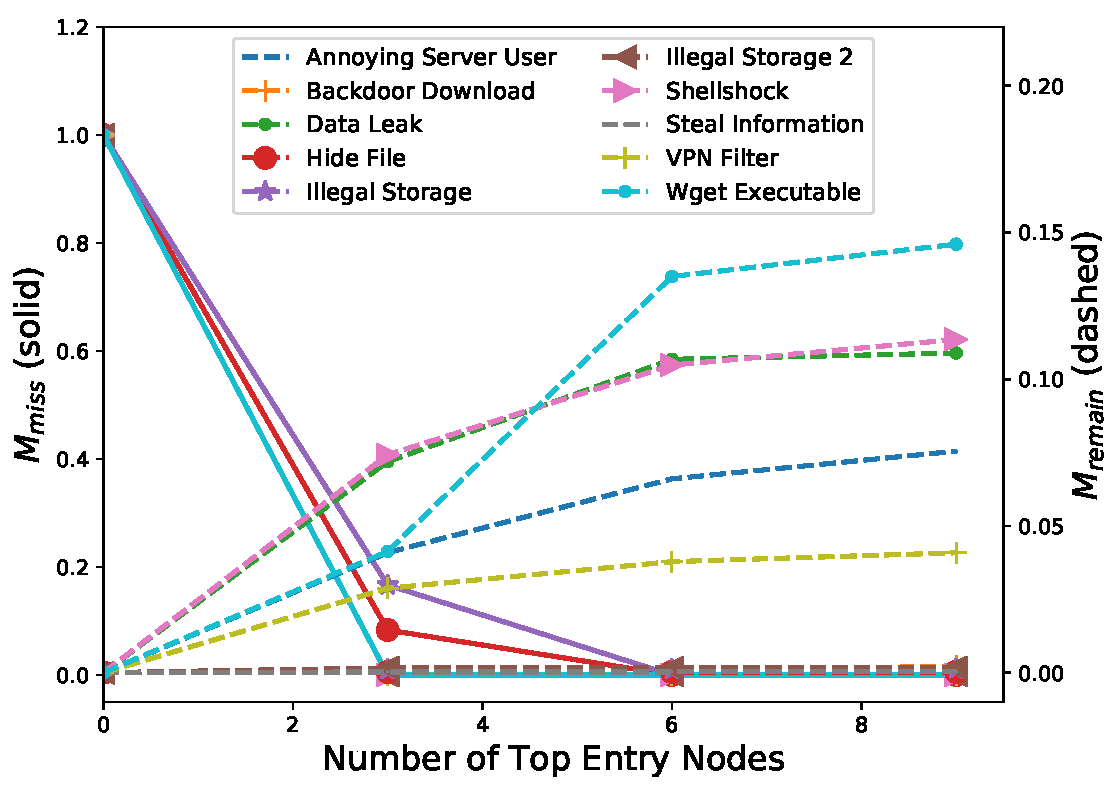
\includegraphics[width=0.47\textwidth]{figs/s&p/rq2-crop.pdf}
    \caption{$M_{miss}$ and $M_{remain}$ using top-ranked entry nodes by considering 3 types of system entities (3, 6, 9 nodes)}
    \label{fig:rq2batch}
\end{figure}
\begin{figure}[t]
    \centering
    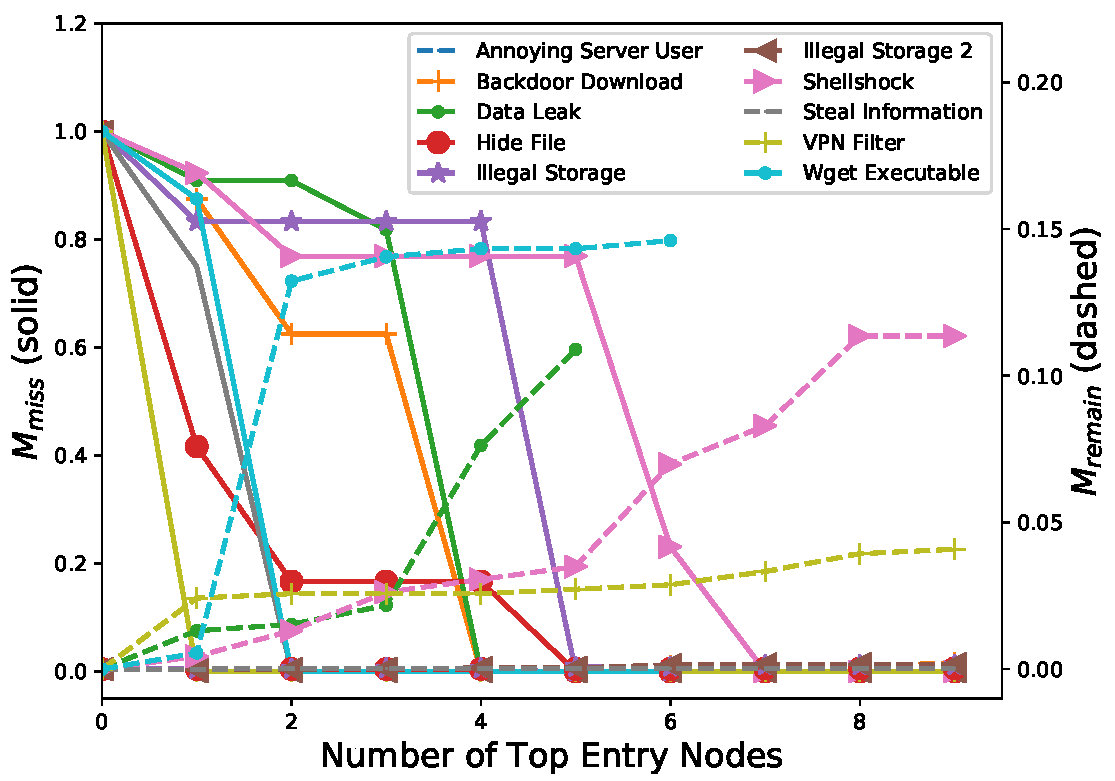
\includegraphics[width=0.47\textwidth]{figs/s&p/rq2m-crop.pdf}
    \caption{$M_{miss}$ and $M_{remain}$ using top-ranked entry nodes without considering the types of system entities (1-9 nodes)}
    \label{fig:rq2single}
\end{figure}

\subsection{RQ2: Impacts of Top-Ranked Entry Nodes}
\label{subsec:rq2}
% Given a dependency graph from a POI event, \tool chooses a number of top-ranked nodes to perform forward causality analysis, and remove the edges that cannot be found via the forward causality analysis.
Intuitively, the more entry nodes \tool uses to perform forward causality analysis, the less likely \tool will incorrectly filter out critical edges.
However, more entry nodes will also cause more non-critical edges to be preserved in the final output graph.
%(\ie overlap of the forward dependency graph and the original backward dependency graph). 
To demonstrate the effectiveness of selecting the top-ranked entry nodes in revealing attack sequences, we show how the increase of the selected top-ranked entry nodes impact the effectiveness of \tool in preserving critical edges and filtering out non-critical edges.
As attack entries may be from different types of system entities, we also compare the effectiveness of two mechanisms in selecting top-ranked entry nodes: one considers the types of system entities and the other does not.

% we first compare \tool with a random approach that randomly selects entry nodes to perform forward causality analysis for filtering. 
% For \tool, we choose top 1, top 2, and top 3 entry nodes from the 3 types of system entities to perform the graph reduction. 
% For the random approach, we choose the 3, 6, and 9 entry nodes for fair comparison.


\myparatight{Evaluation Metrics}
To measure the missing of critical edges, we compute the \emph{missing rate} $M_{miss} = N_{miss} / N_{critical}$, where $N_{miss}$ represents the number of missing critical edges and $N_{critical}$ represents the total number of critical edges (Column ``Critical Edge'' in \cref{tab:stasticalSummary}).
%
To measure the effectiveness of graph reduction, we compute the \emph{remaining rate} $M_{remain} = N_{remain} / N_{total}$, where $N_{remain}$ represents the number of edges in the output graph 
%generated by \tool 
and $N_{total}$ represents the number of edges in the dependency graph after the edge merge (Column ``Edge Mer. \# E'' in \cref{tab:stasticalSummary}).


\eat{
\myparatight{Comparison to Random Approach}
\cref{tab:toolReductionAndMissing} and \cref{tab:rq2random} show the comparison results.
Columns ``1-$M_{miss}$'', ``1-$M_{remain}$'', and ``1-$\# Edge$'' show the average value of $M_{miss}$, the average value of $M_{remain}$, and the average number of edges in the final graph for \tool and the random approach by using the top 1 entry nodes of the 3 types of system entities.
Columns ``2-$M_{miss}$'', ``2-$M_{remain}$'', ``2-$\# Edge$'', ``3-$M_{miss}$'', ``3-$M_{remain}$'', and ``3-$\# Edge$'' show the same metrics for the top 2 and the top 3 entry nodes, respectively. 

As we can see, when the number of entry nodes increases, $M_{miss}$ decreases from $0.02$ to $0.00$ for \tool, but $M_{miss}$ fluctuates for the random approach. 
Another important fact is that when using more entry nodes, the average number of edges remained in the final graph increases from $244.00$ to $268.10$ for \tool, 
while the average number of edges increases from $31,092.21$ to $654,683.47$ for the random approach, which is significantly larger. 
% After the reduction, \tool has about hundreds of edges, but the graph processed by the random approach still has more than 30,000 edges on average. 
Compared with the random approach, \tool can further reduce the edges produced by the random approach by $99.21\%$, $99.96\%$ and $99.95\%$ using the top 1, top 2, and top 3 entry nodes, respectively.
Note that this improvement is not at the cost of losing critical edges for attacks. 
If \tool uses 6 entry nodes (\ie top 2 entry nodes from the 3 system entities), $M_{miss}$ drops to $0.0$.
These results indicates that using irrelevant entry nodes found by the random approach to perform forward causality analysis for filtering is ineffective and may cause the loss of critical edges,
while the top-ranked entry nodes found by \tool contain attack entries so that \tool is effective in revealing attack sequences. 
}

% At the same time, the total number of the edge in the critical component is $268.10$ on average, when \tool uses all the top-three entry nodes. 
% For the random approach, this number is $654,683.47$. 

\myparatight{Impacts on $M_{miss}$ and $M_{remain}$}
As there are 3 types of system entities (\ie processes, files, and network connections), \tool uses the top-ranked entry nodes in different system entity categories
%from all the system entity types 
to perform forward causality analysis (\ie special treatment in \cref{subsubsec:entry-ranking}). 
\cref{fig:rq2batch} shows the values of $M_{miss}$ and $M_{remain}$ with the increases of the used entry nodes.
As expected, when more entry nodes are used, $M_{miss}$ decreases while $M_{remain}$ increases.
This is because performing the forward causality analysis from more entry nodes will make the final graph overlap larger, which is likely to include more critical edges and more non-critical edges. 
We can clearly see that when 6 entry nodes are used (2 nodes from each of the 3 system entity categories), $M_{miss}$ becomes $0.0$.
We further confirm that these 6 entry nodes cover all the attack entries, and more entry nodes merely contribute to the increase of $M_{remain}$.
Another finding is that the dependency impact of the node ranked at the third is about $70\%$ of the top 1 node's dependency impact.
Thus, alternatively, we can use $70\%$ of the top 1 node's dependency impact as the threshold to choose the top-ranked entry nodes for filtering.


\myparatight{Comparison of Two Selection Mechanisms for Top-Ranked Entry Nodes}
We compare \tool's entry node selection mechanism with another mechanism that does not consider system entity categories (\ie selecting top-ranked entry nodes based on their dependency impacts directly).
\cref{fig:rq2single} shows the values of $M_{miss}$ and $M_{remain}$ for this mechanism.
As we can see, for some attacks (\eg the ``VPNFilter'' and ``Wget Executable'' attacks), $M_{miss}$ becomes $0.0$ when the top 1 and the top 2 entry nodes are used,
but some attacks (\eg the ``Shellshock'' attack) requires 7 entry nodes for $M_{miss}$ to become $0.0$.
On the contrary, for all the attacks, the selection mechanism that considers system types can ensure zero-loss of critical edges when 6 entry nodes are used.

\myparatight{Summary}
These results indicate that (1) the top-ranked nodes provided by \tool are effective in preserving critical edges and reducing non-critical edges when the top 2 entry nodes from the 3 types of system entities are used;
(2) the mechanism that considers the types of system entities when choosing the top nodes achieves more stable results for different type of attacks than the one without considering the types of system entities.







\eat{
Considering the complexity of the potential cyberattack, if users want to include more entry points for forward reduction, the change rate of relevance score can be a useful
threshold that may help users select entry node candidates. 
According to our current results, the suggested threshold value for relevance score change is $28\%$. 
That means users can select entry nodes, whose relevance score is bigger than $72\%$ of the highest relevance score in the corresponding category, to do the forward analysis.
}



\eat{

These results demonstrate the superiority of \tool over the random approach,
which is mainly due to the better selection of the entry nodes.
For \tool, the selection of entry nodes is based on the relevance score ranking. 
For the random approach, this selection is a random decision. 
Based on this finding, we can conclude the effectiveness of the graph reduction highly depends on the selection of entry nodes. 


$M_{size}$ is used to measure the graph reduction rate, which is defined as:
\begin{equation}
    M_{size} = \frac{N_{critical}}{N_{merge}}
\end{equation}
$N_{critical}$ is the number of edges in the critical component generated by \tool. $N_{merge}$ is the number of edges after the edge merges. 
A good reduction method should have a small $M_{size}$. If we don't do any graph reduction, $M_{size}$ will be $1.0$.

$M_{miss}$ is used to measure the information loss during the graph reduction. 
Because the corresponding information is represented as edges in dependency graph, we use the critical-edge missing rate to measure the attack information loss. 
$M_{miss}$ is defined as:
\begin{equation}
    M_{miss} = \frac{N_{missing}}{N_{total}}
\end{equation}
$N_{missing}$ is the number of missing critical edges in the critical component generated by \tool. Since we have control over the test environment of these attack cases, we are able to figure out the ground truth of the attack sequences. 
We have the total number of critical edges that should be contained by the critical component, which is represented by $N_{total}$.
Without any filtering, the dependency graph constructed via performing a backward causality analysis from a POI has the $M_{miss}$ being $0.0$.



\tool chooses the top-ranked entry nodes to perform forward causality analysis, and filter the edges that do not appear in the forward causality analysis. 
For this evaluation, we choose the top 3 entry nodes of each category as candidates, and thus we have 9 nodes as candidates in general. 
Given these candidate nodes, we assume that users may pick any of these 9 nodes to perform forward causality analysis for reduction. 
In this evaluation, we use a straightforward way to add entry nodes for forward reduction. 
We add a batch of entry nodes including all 3 kinds of system entities (\ie file, process and IP), the order is according to the rank of relevance score.
Thus, we compute the $M_{size}$ by allowing users to select all top1, top2, or top3 nodes among these candidates, respectively, and then compute $M_{miss}$.


To demonstrate the effectiveness of \tool's graph reduction, we compare \tool with the random  approach. 
For the random approach, all the entry nodes are candidates and the entry nodes used to do the graph reduction are randomly selected. 
We run the random approach for 20 times and compute the average result for these metrics.
For fairness, we will compare the results of \tool and the random approach with the same number of selected nodes, respectively.
}

% We evaluate the graph reduction and critical-edge missing rate, when the attack investigation uses different number of candidates to do the forward reduction. 
% For the dependency graph reduction, if we just simply remove 99.99\% edges of dependency graph, we may have a small graph can be easily analyzed, but it is very possible that we lose all the information about attack. 
% If we only pursue to keep all the attack information, the safest reduction way is just keep all the edges. 
% However, this graph is still too large to be analyzed. 
% The ideal method is try to keep all the critical edges, at the same time remove as much irrelevant edges to POI event as possible.

\begin{table}[t]
\centering
\caption{Average rank of attack entries}
\label{tab:rq3}
\resizebox{0.5\textwidth}{!}{
\begin{tabular}{crrrrr}
\hline
 
\textbf{Attack}        & \multicolumn{1}{c}{\textbf{\tool-{}-}} & \multicolumn{1}{c}{\textbf{\tool-}} & \multicolumn{1}{c}{\textbf{Avg. Proj.}} & \multicolumn{1}{c}{\textbf{Rand.}} & \multicolumn{1}{c}{\textbf{\tool}} \\ \hline
Wget Executable            & 5.50                                     & 12.25                                          & 20.00                                    & 23.45                                    & 5.50                                 \\
Illegal Storage            & 25.00                                    & 13.00                                          & 18.00                                    & 475.99                                   & 7.00                                 \\
Illegal Storage2           & 1.00                                     & 1.00                                           & 1.00                                     & 1,893.66                                 & 1.00                                 \\
Hide File                  & 22.00                                    & 10.50                                          & 13.50                                    & 17,284.72                                & 1.00                                 \\
Steal Information          & 11.00                                    & 3.50                                           & 7.00                                     & 17,304.32                                & 11.00                                \\
Backdoor Download          & 3.50                                     & 3.50                                           & 7.50                                     & 76.57                                    & 6.50                                 \\
Annoying Server User\_user & 5.00                                     & 5.00                                           & 13.00                                    & 15.82                                    & 4.00                                 \\
Shellshcok                 & 11.00                                    & 19.00                                          & 13.00                                    & 22.63                                    & 11.00                                \\
Dataleak                   & 35.00                                    & 9.00                                           & 9.00                                     & 48.34                                    & 8.00                                 \\
VPN Filter                 & 46.00                                    & 34.00                                          & 8.00                                     & 236.77                                   & 7.00                                 \\
Five Dir. Case1            & 5.00                                     & 5.00                                           & 5.00                                     & 115.50                                   & 5                                    \\
Five Dir. Case3            & 1                                        & 1                                              & 1                                        & 327.10                                   & 2                                    \\
Theia Case1                & 1                                        & 1                                              & 1                                        & 88956.7                                  & 1                                    \\
Theia Case3                & 1                                        & 2                                              & 1                                        & 70610.5                                  & 1                                    \\
Trace Case5                & 2                                        & 2                                              & 2                                        & 10.1                                     & 2                                    \\
AVG                        & 11.67                                    & 8.12                                           & 8.00                                     & 13,160.14                                & 4.87                                 \\ \hline
\end{tabular}
}
\end{table}

%\begin{table}[!t]
\centering
\caption{Performance statistics of \tool}
\label{tab:runtime}
\resizebox{0.48\textwidth}{!}{%
\begin{tabular}{|l|r|r|r|r|r|}
\hline
            \textbf{Case}         & \textbf{Causality} & \textbf{Edge Merge} & \textbf{Node Split} & \textbf{Weight} & \textbf{Rep. Propagation} \\ \hline
penetration-c1       & 0.088                     & 0.001           & 0.002             & 0.013                          & 0.069                              \\ \hline
penetration-c2       & 0.086                     & 0.000           & 0.000             & 0.027                          & 0.001                              \\ \hline
password-crack-c1    & 0.186                     & 0.001           & 0.000             & 0.009                          & 0.000                              \\ \hline
password-crack-c2    & 0.183                     & 0.007           & 0.001             & 0.015                          & 0.001                              \\ \hline
password-crack-c3    & 0.256                     & 0.152           & 0.001             & 0.022                          & 0.000                              \\ \hline
data-leakage         & 0.568                     & 0.450           & 0.019             & 1.697                          & 0.031                              \\ \hline
command-injection-c1 & 0.246                     & 0.001           & 0.001             & 0.020                          & 0.000                              \\ \hline
command-injection-c2 & 0.215                     & 0.025           & 0.006             & 0.668                          & 0.008                              \\ \hline
vpnfilter-c1         & 0.179                     & 0.002           & 0.000             & 0.006                          & 0.000                              \\ \hline
vpnfilter-c2         & 0.162                     & 0.007           & 0.000             & 0.053                          & 0.000                              \\ \hline
\textbf{avg}         & \textbf{0.21}            & \textbf{0.06}  & \textbf{0.003}   & \textbf{0.25}                 & \textbf{0.01}                     \\ \hline
\end{tabular}
}
\end{table}


\eat{
\begin{figure}[t]
    \centering
    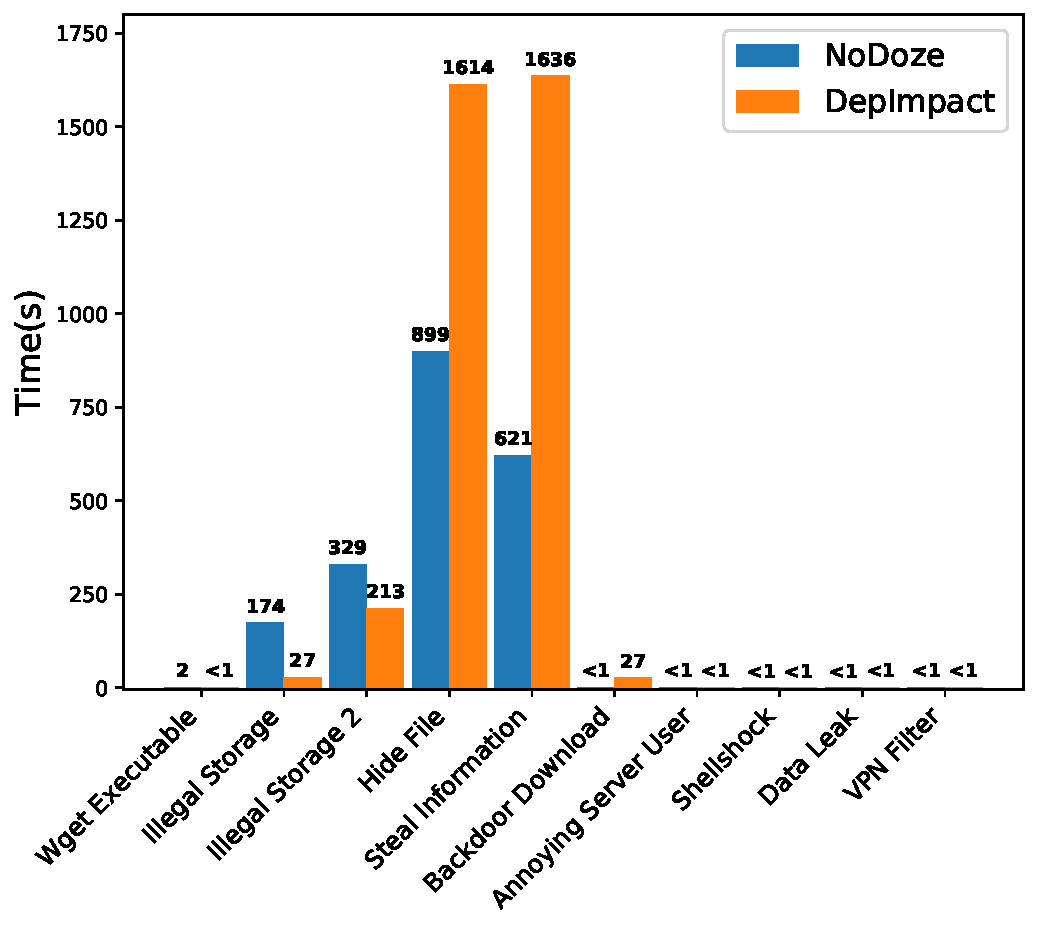
\includegraphics[width=0.48\textwidth]{figs/s&p/rq4.pdf}
    \caption{Runtime performance of \tool and NoDoze}
    \label{fig:rq4compare}
\end{figure}
}

\subsection{RQ4: System Performance}

To understand the performance of \tool, we measure the execution time of each step in \tool, as shown in \cref{tab:rq4performance}.
On average, \tool takes $343.84s$ to finish
%the processing and computation for one 
analyzing an attack (\ie weight computation and impact propagation) and dependency graph construction requires $65.83s$ (\ie causality analysis and edge merge).
We next compare \tool with the average-projection approach and NoDoze.
We exclude the comparison of the execution times for the common steps (causality analysis and edge merge).


% We compare \tool with the average-projection approach for dependency weight computation and dependency impact propagation, since they share the same steps for causality analysis and edge merge. 
From the comparison results of \tool and the average-projection approach in \cref{tab:rq4performance}, we observe that 
(1) \tool takes more time for dependency weight computation ($\sim120s$) because \tool uses the Multi-KMeans++ clustering and LDA to find the optimal projection vector;
(2) \tool takes less time for dependency impact propagation. The reason is because the dependency weights computed by \tool are much more discriminative, and hence the score propagation can converge faster.
%but the shorter time for the average-projection approach in dependency weight computation is offsetted by the time needed for score propagation. 
As a result, \tool reduces the execution time by $71.94\%$ when compared with the average-projection approach. 

% We also compare the execution time of \tool (dependency weight computation plus dependency impact propagation) with the execution time of NoDoze (anomaly score computation), since they share the same causality analysis and edge merge steps. We only compare the different parts: weight computation and impact propagation.
From the comparison results of \tool and Nodoze in \cref{tab:rq4performance}, we can see \tool need $343.84s$ to finish the weight computation and impact propagation, NoDoze need $144.15s$ to finish the s anomaly score computation.
%
In particular, while \tool requires more time for processing the 2 attacks whose dependency graphs have more than 3 million edges (\ie the ``Hide File'' attack and the ``Steal information'' attack), \tool produces much smaller graphs ($\sim800$ edges) than NoDoze ($>20,000$ edges).
On average, \tool needs $343.84$s to finish the dependency weight computation and the dependency impact propagation, and NoDoze needs $144.15$s to finish the anomaly score computation ($409.67s$ v.s. $209.98s$ for the whole analysis).
%
Thus, \tool and NoDoze have similar runtime performance for most of the attacks, and NoDoze is more efficient for certain attacks but achieves much lower graph reduction. 



\eat{
Also, the results in \cref{subsec:rq3} show that \tool achieves better ranking for the attack entries than the average-projection approach, and we want to know whether it is at the cost of more computation efforts.
The results are shown in \cref{tab:rq4performance}.



To understand the performance of \tool in investigating real attacks, we measure the execution time of \tool on the attack cases.
\tool starts the computation by parsing a log ($92.252s$ averagely) and building a global graph representation ($3.277s$ averagely).
\cref{tab:runtime} shows the execution time for the remaining components of \tool. 
Besides the steps shown in the preprocessing step, \emph{Causality Analysis}, \emph{Edge Merge}, and \emph{Node split} require $0.21s$, $0.06s$, and $0.003$ on average. 
Note that \emph{Weight Computation} and \emph{Reputation Propagation} only requires $0.25s$ and $0.01s$ on average.
In summary, the total time for running an analysis is about $2$ minutes, but the major cost (\ie log parsing) can be improved by adopting caching or database indexing~\cite{gao2018aiql}.
}

% \subsection{Case Study}
% \begin{figure*}
%     \centering
%     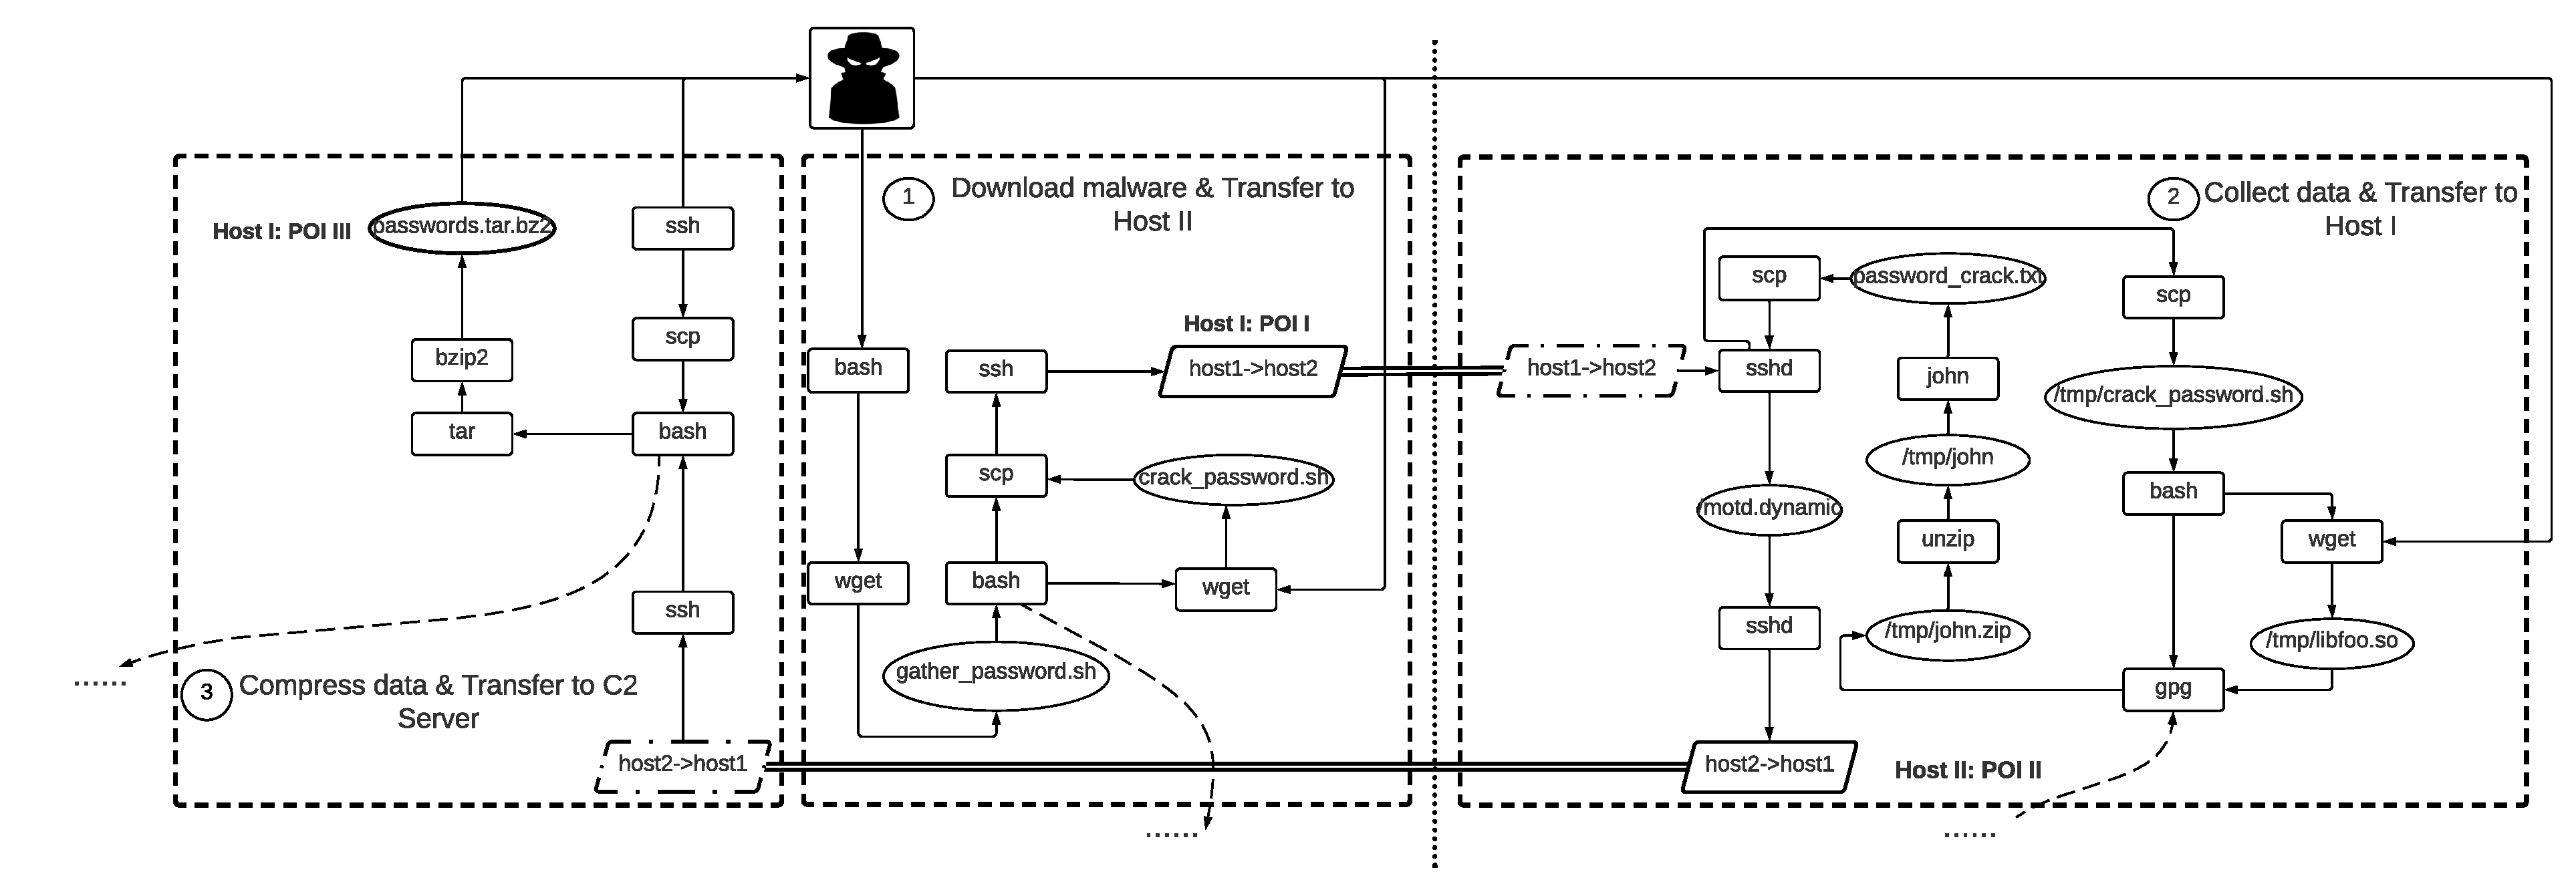
\includegraphics[width=0.98\textwidth]{figs/2021usenix/multihost.pdf}
%     \caption{Caption}
%     \label{fig:my_label}
% \end{figure*}







